%%%%%%%%%%%%%%%%%%%%%%%%%%%%%%%%%%%%%%%%%%%%%%%%%%%%%%%%%%%%%%%%%%%%%%%%%%%%%%%%%%
\begin{frame}[fragile]\frametitle{}

\begin{center}
{\Large Named Entity Recognition}
\end{center}
\end{frame}

%%%%%%%%%%%%%%%%%%%%%%%%%%%%%%%%%%%%%%%%%%%%%%%%%%%%%%%%%%%%%%%%%%%%%%%%%%%%%%%%%%
\begin{frame}[fragile]\frametitle{Introduction}
In NLP, NER is a method of extracting the relevant information from a large corpus and classifying those entities into predefined categories such as location, organization, name and so on.

  \begin{center}
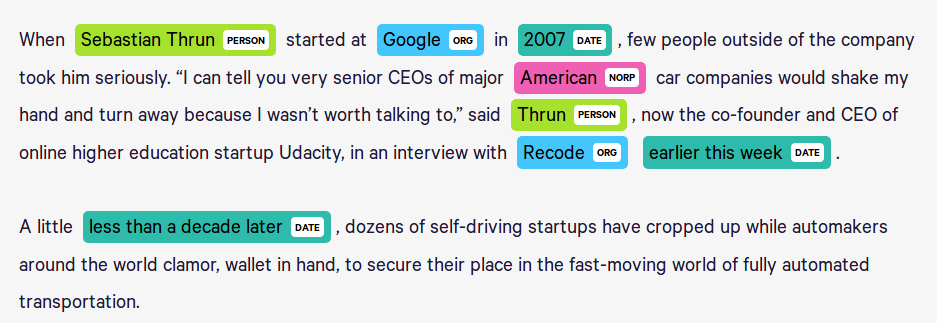
\includegraphics[width=\linewidth,keepaspectratio]{ner11}
\end{center}


	{\tiny (Ref: Complete Tutorial on Named Entity Recognition (NER) using Python and Keras - Akshay Chavan)}
\end{frame}




%%%%%%%%%%%%%%%%%%%%%%%%%%%%%%%%%%%%%%%%%%%%%%%%%%%%%%%%%%%%%%%%%%%%%%%%%%%%%%%%%%
\begin{frame}[fragile]\frametitle{The who, where, when \& how much in a sentence}
The task: identify atomic elements of information in text
  \begin{itemize}
  \item Person names
  \item Company/organization names
  \item Locations
  \item Dates \& times
  \item Percentages
  \item Monetary amounts
  \end{itemize}
  \begin{center}
\includegraphics[width=0.8\linewidth,keepaspectratio]{ner2}
\end{center}
\end{frame}


%%%%%%%%%%%%%%%%%%%%%%%%%%%%%%%%%%%%%%%%%%%%%%%%%%%%%%%%%%%%%%%%%%%%%%%%%%%%%%%%%%
\begin{frame}[fragile]\frametitle{Example}

  \begin{center}
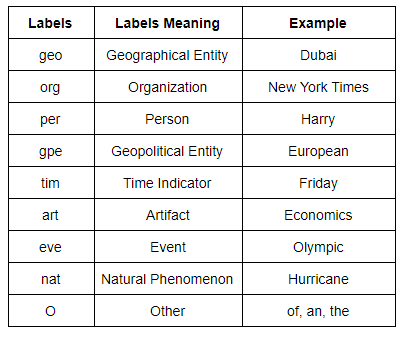
\includegraphics[width=0.6\linewidth,keepaspectratio]{ner12}
\end{center}


	{\tiny (Ref: Complete Tutorial on Named Entity Recognition (NER) using Python and Keras - Akshay Chavan)}
\end{frame}



%%%%%%%%%%%%%%%%%%%%%%%%%%%%%%%%%%%%%%%%%%%%%%%%%%%%%%%%%%%%%%%%%%%%%%%%%%%%%%%%%%
\begin{frame}[fragile]\frametitle{Difficulties}
  \begin{itemize}
  \item Too numerous to include in dictionaries
  \item Changing constantly: new names invent unknown words
  \item Appear in many variant forms: e.g. John Smith, Mr Smith, John
  \item Subsequent occurrences might be abbreviated
  \item List search/matching does't perform well
  \end{itemize}
\end{frame}

%%%%%%%%%%%%%%%%%%%%%%%%%%%%%%%%%%%%%%%%%%%%%%%%%%%%%%%%%%%%%%%%%%%%%%%%%%%%%%%%%%
\begin{frame}[fragile]\frametitle{Concept}
Whether a phrase is a proper name, and what name class it has, depends on

  \begin{itemize}
  \item Internal structure:``Mr. London'' 
  \item Context:``The new location, London, will make a better place.''
  \end{itemize}
\end{frame}

%%%%%%%%%%%%%%%%%%%%%%%%%%%%%%%%%%%%%%%%%%%%%%%%%%%%%%%%%%%%%%%%%%%%%%%%%%%%%%%%%%
\begin{frame}[fragile]\frametitle{Applications}
  \begin{itemize}
  \item Information Extraction:  relations are associations between named entities
  \item Named entities can be indexed, linked off, etc.
  \item Sentiment can be attributed to companies or products
  \item Summary generation
  \item Machine Translation
  \item Document organization/classification
  \item Increase accuracy of Internet search results (location Clinton/South Carolina vs. President Clinton)
  \item For question answering, answers are often named entities
  \end{itemize}
\end{frame}

%%%%%%%%%%%%%%%%%%%%%%%%%%%%%%%%%%%%%%%%%%%%%%%%%%%%%%%%%%%%%%%%%%%%%%%%%%%%%%%%%%
\begin{frame}[fragile]\frametitle{Standard Approaches}
  \begin{itemize}
  \item Hand-written regular expressions:  Perhaps stacked
  \item Using classifiers: Naïve Bayes, Maxent models
  \item Sequence models:HMMs, CRFs
  \end{itemize}
	
\begin{center}
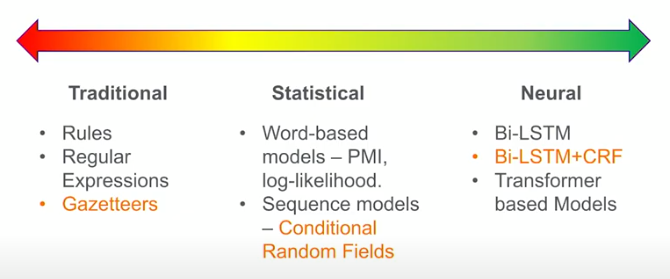
\includegraphics[width=0.8\linewidth,keepaspectratio]{ner17}
\end{center}

Note: Gazetteers are dictionaries or lookup lists.

{\tiny (Ref: Sujit Pal: Building Named Entity Recognition Models Efficiently Using NERDS | PyData LA 2019)}
	
\end{frame}

%%%%%%%%%%%%%%%%%%%%%%%%%%%%%%%%%%%%%%%%%%%%%%%%%%%%%%%%%%%%%%%%%%%%%%%%%%%%%%%%%%
\begin{frame}[fragile]\frametitle{The hand-crafted/Rule-based approach}
Uses hand-written context-sensitive reduction rules:
  \begin{itemize}
  \item For certain restricted, common types of entities in unstructured 
text, simple regex patterns also usually work.
  \item Finding (US) phone numbers
  \item \lstinline| (?:\(?[0-9]{3}\)?[ -.])?[0-9]{3}[ -.]?[0-9]{4}|
  \item Title capitalized word : title person\_name compare ``Mr. Jones'' vs. ``Mr. Ten-Percent'' : no rule without exceptions
  \item  person\_name, ``the'' adj* ``CEO of'' organization ``Fred Smith, the young dynamic CEO of BlubbCo'' : ability to grasp non-local patterns
  \end{itemize}
  Plus help from databases of known named entities

\end{frame}

% %%%%%%%%%%%%%%%%%%%%%%%%%%%%%%%%%%%%%%%%%%%%%%%%%%%%%%%%%%%%%%%%%%%%%%%%%%%%%%%%%%
% \begin{frame}[fragile]\frametitle{Word Features}
% Easily determinable token properties:
% \begin{center}
% 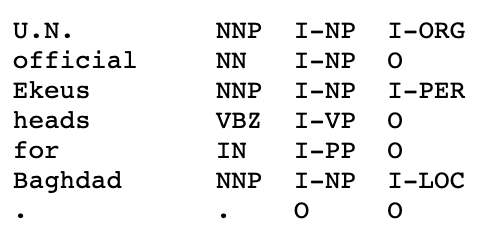
\includegraphics[width=\linewidth,keepaspectratio]{ner1}
% \end{center}
% \end{frame}

% %%%%%%%%%%%%%%%%%%%%%%%%%%%%%%%%%%%%%%%%%%%%%%%%%%%%%%%%%%%%%%%%%%%%%%%%%%%%%%%%%%
% \begin{frame}[fragile]\frametitle{MUC: the NLP genesis of IE}
  % \begin{itemize}
  % \item DARPA funded significant efforts in IE in the early to mid 1990s
  % \item Message Understanding Conference (MUC) was an annual event/competition where results were presented.
  % \item Focused on extracting information from news articles: Terrorist events, Industrial joint ventures, Company management changes
  % \item Starting off, all rule-based, gradually moved to ML
  % \end{itemize}
% \end{frame}

% %%%%%%%%%%%%%%%%%%%%%%%%%%%%%%%%%%%%%%%%%%%%%%%%%%%%%%%%%%%%%%%%%%%%%%%%%%%%%%%%%%
% \begin{frame}[fragile]\frametitle{Example from MUC-7}
% Delimit the named entities in a text and tag them with NE categores:

  % \begin{lstlisting}
% <ENAMEX TYPE=``LOCATION''>Italy</ENAMEX>'s business world was rocked by
% the announcement <TIMEX TYPE=``DATE''>last Thursday</TIMEX> that Mr.
% <ENAMEX TYPE=``PERSON''>Verdi</ENAMEX> would leave his job as vice-president
% of <ENAMEX TYPE=``ORGANIZATION''>Music Masters of Milan, Inc</ENAMEX> 
% to become operations director of  
% <ENAMEX TYPE=``ORGANIZATION''>Arthur Andersen</ENAMEX>.
  % \end{lstlisting}
  
  % \begin{itemize}
  % \item ``Milan'' is part of organization name
  % \item ``Arthur Andersen'' is a company 
  % \item ``Italy'' is sentence-initial : capitalization useless
  % \end{itemize}
% \end{frame}

% %%%%%%%%%%%%%%%%%%%%%%%%%%%%%%%%%%%%%%%%%%%%%%%%%%%%%%%%%%%%%%%%%%%%%%%%%%%%%%%%%%
% \begin{frame}[fragile]\frametitle{Hand-written Information Extraction}
% For unstructured human-written text, some NLP may help
  % \begin{itemize}
  % \item Part-of-speech (POS) tagging: Mark each word as a noun, verb, preposition, etc.
  % \item Syntactic parsing: Identify phrases: NP, VP, PP
  % \item Semantic word categories (e.g. from WordNet): KILL: kill, murder, assassinate, strangle, suffocate
  % \end{itemize}
% \end{frame}



%%%%%%%%%%%%%%%%%%%%%%%%%%%%%%%%%%%%%%%%%%%%%%%%%%%%%%%%%%%%%%%%%%%%%%%%%%%%%%%%%%
\begin{frame}[fragile]\frametitle{Methods for Sequence Labeling}
Typically the following methods are used for NER:
  \begin{itemize}
  \item Hidden Markov Model (HMM)
  \item Maximum Entropy Classifier (MaxEnt)
  \item Maximum Entropy Markov Model (MEMM)
  \item Conditional Random Fields (CRF)
  \end{itemize}
These are all classifiers (i.e., supervised learning) which model sequences (rather than individual random variables)
\end{frame}

%%%%%%%%%%%%%%%%%%%%%%%%%%%%%%%%%%%%%%%%%%%%%%%%%%%%%%%%%%%%%%%%%%%%%%%%%%%%%%%%%%
\begin{frame}[fragile]\frametitle{Sequence approach}
Training
  \begin{itemize}
  \item  Collect a set of representative training documents
  \item  Label each token for its entity class or other (O)
  \item  Design feature extractors appropriate to the text and classes 3. Design feature extractors appropriate to the text and classes
  \item  Train a sequence classifier to predict the labels from the data
  \end{itemize}
Testing  
  \begin{itemize}
  \item  Receive a set of testing documents
  \item  Run sequence model inference to label each token
  \item  Appropriately output the recognized entities
  \end{itemize}
\end{frame}

% %%%%%%%%%%%%%%%%%%%%%%%%%%%%%%%%%%%%%%%%%%%%%%%%%%%%%%%%%%%%%%%%%%%%%%%%%%%%%%%%%%
% \begin{frame}[fragile]\frametitle{Features}
  % \begin{itemize}
  % \item History $h_t$: information derivable from the corpus relative to a token $t$:
    % \begin{itemize}
  % \item text window around token $w-i$, e.g. $w_{i-2},\ldots,w_{i+2}$
  % \item word features of these tokens
  % \item POS, other complex features
    % \end{itemize}
  % \item Binary features: yes/no-questions on history used by models to determine probabilities of
  % \item Futures: name classes

  % \end{itemize}
% \end{frame}
%%%%%%%%%%%%%%%%%%%%%%%%%%%%%%%%%%%%%%%%%%%%%%%%%%%%%%%%%%%%%%%%%%%%%%%%%%%%%%%%%%
\begin{frame}[fragile]\frametitle{Features for sequence labeling}
  \begin{itemize}
  \item Words:
  \begin{itemize}
  \item Current word (essentially like a learned dictionary)
  \item Previous/next word (context)
  \end{itemize}
  \item Other kinds of inferred linguistic classification: Part-of-speech tags
  \item Label context: Previous (and perhaps next) label
  \item Word Shapes: Map words to simplified representation that encodes attributes such as length, capitalization, numerals, Greek letters, internal punctuation, etc.
\begin{center}
\includegraphics[width=0.4\linewidth,keepaspectratio]{ner4}
\end{center}
  \end{itemize}
\end{frame}

%%%%%%%%%%%%%%%%%%%%%%%%%%%%%%%%%%%%%%%%%%%%%%%%%%%%%%%%%%%%%%%%%%%%%%%%%%%%%%%%%%
\begin{frame}[fragile]\frametitle{BIO or IOB format}

\begin{center}
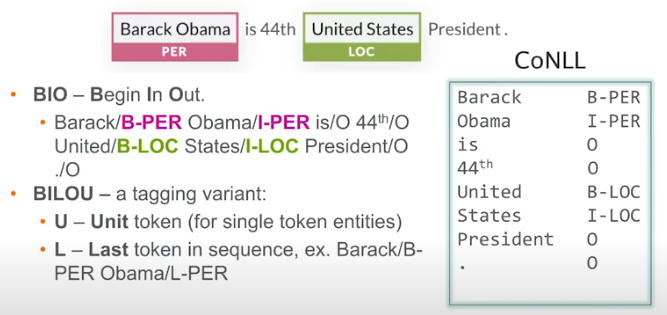
\includegraphics[width=\linewidth,keepaspectratio]{ner18}
\end{center}

{\tiny (Ref: Sujit Pal: Building Named Entity Recognition Models Efficiently Using NERDS | PyData LA 2019)}

\end{frame}

%%%%%%%%%%%%%%%%%%%%%%%%%%%%%%%%%%%%%%%%%%%%%%%%%%%%%%%%%%%%%%%%%%%%%%%%%%%%%%%%%%
\begin{frame}[fragile]\frametitle{Features and Output Data format}

\begin{center}
\includegraphics[width=0.8\linewidth,keepaspectratio]{ner3}

\includegraphics[width=\linewidth,keepaspectratio]{ner5}
\end{center}
\end{frame}

%%%%%%%%%%%%%%%%%%%%%%%%%%%%%%%%%%%%%%%%%%%%%%%%%%%%%%%%%%%%%%%%%%%%%%%%%%%%%%%%%%
\begin{frame}[fragile]\frametitle{Dataset example}

CoNLL-2003

  \begin{itemize}
  \item CoNLL - Conference on Natural Language Learning by the ACL's Special Interest Group on Natural Language Learning
  \item Shared Task: Language-Independent Named Entity Recognition
  \item Goal: Identify boundaries and types of named entities
\begin{center}
\includegraphics[width=0.5\linewidth,keepaspectratio]{ner9}
\end{center}
\item Inputs: $x = (x_1,\ldots, x_n)$
\item Labels: $y = (y_1,\ldots, y_n)$
\item Typical goal: Given $x$, predict $y$

  \end{itemize}
\end{frame}

%%%%%%%%%%%%%%%%%%%%%%%%%%%%%%%%%%%%%%%%%%%%%%%%%%%%%%%%%%%%%%%%%%%%%%%%%%%%%%%%%%
\begin{frame}[fragile]\frametitle{}

\begin{center}
{\Large Algorithms}
\end{center}
\end{frame}



% %%%%%%%%%%%%%%%%%%%%%%%%%%%%%%%%%%%%%%%%%%%%%%%%%%%%%%%%%%%%%%%%%%%%%%%%%%%%%%%%%%
% \begin{frame}[fragile]\frametitle{Maximum Entropy Markov Model (MEMM)}
  % \begin{itemize}
  % \item (MEMM) classifier makes a single decision at a time, conditioned on evidence from observations and previous decisions.
  % \item Scoring individual labeling decisions is no more complex than standard classification decisions. Using features for classification.
  % \end{itemize}
% \begin{center}
% \includegraphics[width=\linewidth,keepaspectratio]{ner6}
% \end{center}
% \end{frame}

% %%%%%%%%%%%%%%%%%%%%%%%%%%%%%%%%%%%%%%%%%%%%%%%%%%%%%%%%%%%%%%%%%%%%%%%%%%%%%%%%%%
% \begin{frame}[fragile]\frametitle{Hidden Markov Models (HMMs)}
% \begin{center}
% \includegraphics[width=0.9\linewidth,keepaspectratio]{ner10}
% \end{center}
% \end{frame}

% %%%%%%%%%%%%%%%%%%%%%%%%%%%%%%%%%%%%%%%%%%%%%%%%%%%%%%%%%%%%%%%%%%%%%%%%%%%%%%%%%%
% \begin{frame}[fragile]\frametitle{Viterbi Inference}
  % \begin{itemize}
  % \item Dynamic programming or memoization.
  % \item Requires small window of state influence (e.g., past two states are relevant).
  % \item Advantage:: Exact: the global best sequence is returned.
  % \item Disadvantage: Harder to implement long-distance state-state interactions (but beam inference tends not
% to allow long-distance resurrection of sequences anyway).
  % \end{itemize}
% \begin{center}
% \includegraphics[width=\linewidth,keepaspectratio]{ner7}
% \end{center}
% \end{frame}

% %%%%%%%%%%%%%%%%%%%%%%%%%%%%%%%%%%%%%%%%%%%%%%%%%%%%%%%%%%%%%%%%%%%%%%%%%%%%%%%%%%
% \begin{frame}[fragile]\frametitle{Viterbi Inference}
% \begin{center}
% \includegraphics[width=\linewidth,keepaspectratio]{ner8}
% \end{center}
% \end{frame}

% %%%%%%%%%%%%%%%%%%%%%%%%%%%%%%%%%%%%%%%%%%%%%%%%%%%%%%%%%%%%%%%%%%%%%%%%%%%%%%%%%%
% \begin{frame}[fragile]\frametitle{Viterbi Inference}
  % \begin{itemize}
  % \item Create an array, with columns corresponding to inputs, rows corresponding to possible states
  % \item Sweep through the array in one pass filling the columns left to right using our transition probs and observations probs
  % \item Dynamic programming key is that we need only store the MAX prob path to each cell, (not all paths).
  % \end{itemize}
% \end{frame}

%%%%%%%%%%%%%%%%%%%%%%%%%%%%%%%%%%%%%%%%%%%%%%%%%%%%%%%%%%%%%%%%%%%%%%%%%%%%%%%%%%
\begin{frame}[fragile]\frametitle{Conditional Random Fields (CRFs)}
  \begin{itemize}
  \item CRFs are used for predicting the sequences that use the contextual information to add information which will be used by the model to make a correct prediction.
	\item The output sequence is modeled as the normalized product of the feature function.
	\item Actually its similar to basic Logistic Regression, done for each token, with a custom feature lists, having info of the context.
  \end{itemize}
	
\begin{center}
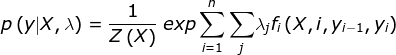
\includegraphics[width=0.5\linewidth,keepaspectratio]{ner13}
\end{center}
\end{frame}

%%%%%%%%%%%%%%%%%%%%%%%%%%%%%%%%%%%%%%%%%%%%%%%%%%%%%%%%%%%%%%%%%%%%%%%%%%%%%%%%%%
\begin{frame}[fragile]\frametitle{Task specific predictions}
  \begin{itemize}
  \item Inputs: words (e.g., Bill, Microsoft, etc)
	\item Outputs: Tags (e.g. PERSON, ORG, etc)
	\item Features: context (neighboring words, POS, etc)
	\item Why Probabilistic Graphical Model like CRF? : features are correlated. Not like Naive Bayes.
	\item So, instead of modeling JOINT distribution of X and Y, CRF is trying to model CONDITIONAL distribution of Y given X. So, correlations amongst Xs are irrelevant here.
  \end{itemize}
	
\begin{center}
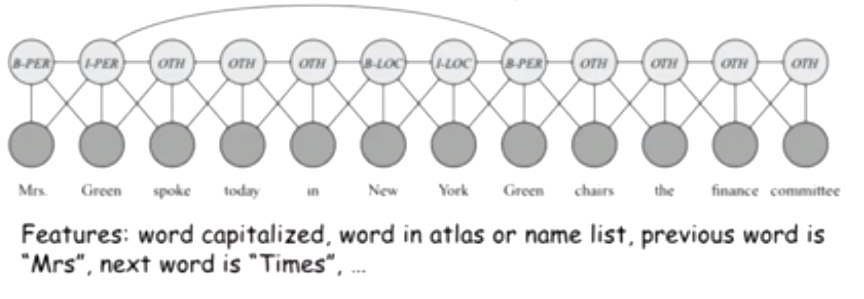
\includegraphics[width=0.5\linewidth,keepaspectratio]{ner25}
\end{center}


	{\tiny (Ref: Conditional Random Fields - Stanford University - Daphne Koller)}
	
	
\end{frame}

%%%%%%%%%%%%%%%%%%%%%%%%%%%%%%%%%%%%%%%%%%%%%%%%%%%%%%%%%%%%%%%%%%%%%%%%%%%%%%%%%%
\begin{frame}[fragile]\frametitle{Feature Preparation for CRF}

\begin{center}
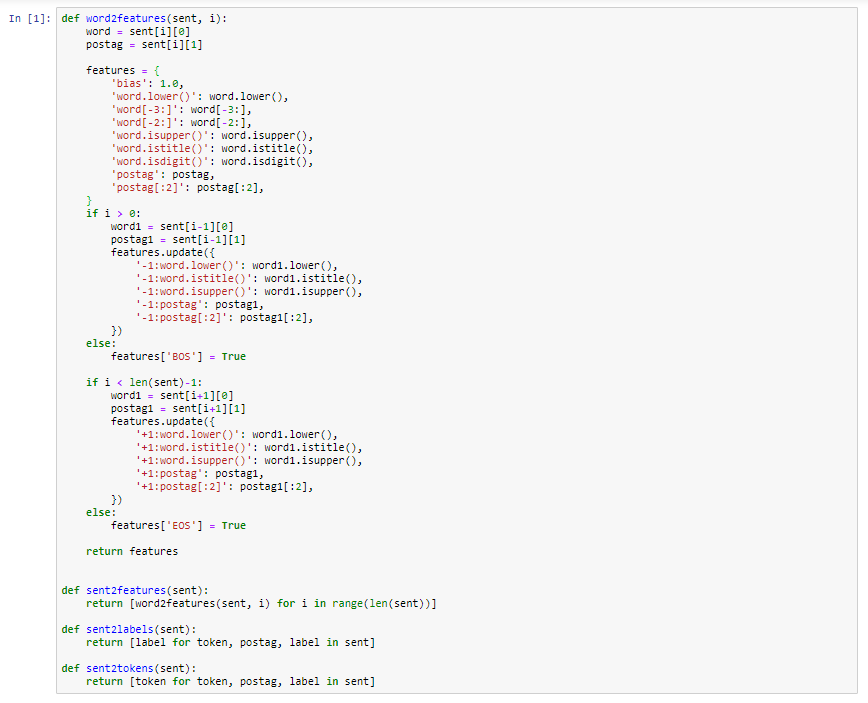
\includegraphics[width=0.8\linewidth,keepaspectratio]{ner14}
\end{center}

\end{frame}

%%%%%%%%%%%%%%%%%%%%%%%%%%%%%%%%%%%%%%%%%%%%%%%%%%%%%%%%%%%%%%%%%%%%%%%%%%%%%%%%%%
\begin{frame}[fragile]\frametitle{Training the model with scikit-learn}

\begin{center}
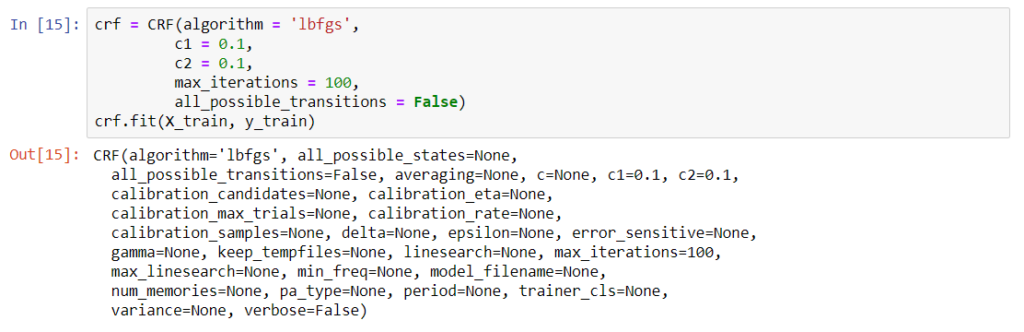
\includegraphics[width=\linewidth,keepaspectratio]{ner15}
\end{center}

\end{frame}

%%%%%%%%%%%%%%%%%%%%%%%%%%%%%%%%%%%%%%%%%%%%%%%%%%%%%%%%%%%%%%%%%%%%%%%%%%%%%%%%%%
\begin{frame}[fragile]\frametitle{Evaluating the model  performance}

\begin{center}
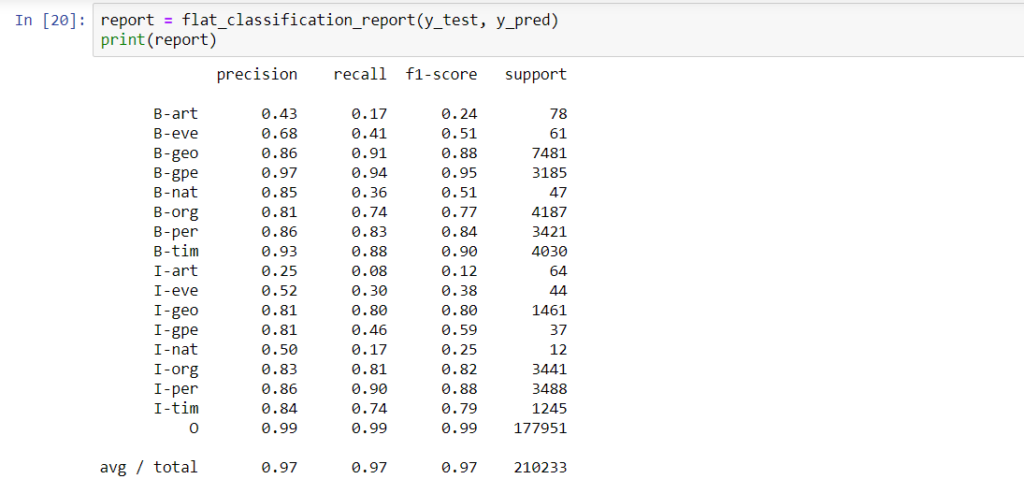
\includegraphics[width=\linewidth,keepaspectratio]{ner16}
\end{center}

\end{frame}

%%%%%%%%%%%%%%%%%%%%%%%%%%%%%%%%%%%%%%%%%%%%%%%%%%%%%%%%%%%%%%%%%%%%%%%%%%%%%%%%%%
\begin{frame}[fragile]\frametitle{Summary}
  \begin{itemize}
  \item CRF is parametrized the same as a Gibbs distribution but normalized differently.
	\item Generalizes Logistic Regression Model.
  \end{itemize}
	

	{\tiny (Ref: Conditional Random Fields - Stanford University - Daphne Koller)}
	
	
\end{frame}



%%%%%%%%%%%%%%%%%%%%%%%%%%%%%%%%%%%%%%%%%%%%%%%%%%%%%%%%%%%%%%%%%%%%%%%%%%%%%%%%%%
\begin{frame}[fragile]\frametitle{}

\begin{center}
{\Large Conclusions}
\end{center}
\end{frame}


%%%%%%%%%%%%%%%%%%%%%%%%%%%%%%%%%%%%%%%%%%%%%%%%%%%%%%%%%%%%%%%%%%%%%%%%%%%%%%%%%%
\begin{frame}[fragile]\frametitle{Hand-crafted vs. Automated }
Hand-made systems:
  \begin{itemize}
  \item Can achieve higher performance than ML systems
  \item Non-local phenomena best handled by regular expressions
  \item Several person-months for rule-writing, requires experienced linguists
  \item Rules depend on specific properties of language, domain \& text format  
  \item Manual adaption necessary when domain changes
  \item Re-write rules for other languages
  \end{itemize}
\end{frame}

%%%%%%%%%%%%%%%%%%%%%%%%%%%%%%%%%%%%%%%%%%%%%%%%%%%%%%%%%%%%%%%%%%%%%%%%%%%%%%%%%%
\begin{frame}[fragile]\frametitle{Hand-crafted vs. Automated }
Automated approaches:
  \begin{itemize}
  \item Train on human-annotated texts
  \item No expensive computational linguists needed
  \item 1,00,000 words can be tagged in 1-3 days
  \item Ideally, no manual work required for domain changes
  \item Easier to port to other languages
  \item Features are locally limited
  \end{itemize}
\end{frame}

%%%%%%%%%%%%%%%%%%%%%%%%%%%%%%%%%%%%%%%%%%%%%%%%%%%%%%%%%%%%%%%%%%%%%%%%%%%%%%%%%%
\begin{frame}[fragile]\frametitle{Evaluation for NER }
  \begin{itemize}
  \item Recall and precision are straightforward for tasks like IR and text 
categorization, where there is only one grain size (documents)
  \item The measure behaves a bit funnily for IE/NER when there are 
boundary errors (which are common):
  \item First Bank of Chicago announced earnings
  \item This counts as both a FP and a FN
  \item Selecting nothing would have been better
  \item Some other metrics (e.g., MUC scorer) give partial credit (according to complex rules)
  \end{itemize}
\end{frame}
